\documentclass[../../main.tex]{subfiles}
\graphicspath{{../../image/}{../../figure/}}
\begin{document}

\section{定常平面等熵气流}\label{section:ch18-定常平面等熵气流}

转向二维空间中的守恒律方程组，我们考虑气体的定常平面等熵流动，气体的状态方程为 $p(\rho)$，满足 $p'(\rho)>0$，$p''(\rho)>0$。在 Euler 坐标中，密度与速度不依赖于时间。于是，以 $(x,y)$ 记空间变量、$(u,v)$ 记速度分量，无体积力时二维形式的 Euler 方程组\eqref{align:ch03-等熵Euler}退化为
\begin{align}
\begin{cases}
\partial_x(\rho u)+\partial_y(\rho v)=0\\
\partial_x(\rho u^2+p(\rho))+\partial_y(\rho uv)=0\\
\partial_x(\rho uv)+\partial_y(\rho v^2+p(\rho))=0.
\end{cases}
\label{align:ch18-1821}
\end{align}
声速为
\begin{align}
c=\sqrt{p'(\rho)}.
\label{align:ch18-1822}
\end{align}
沿 $x$-方向（而非 $t$-方向）检验双曲性，可得特征值
\begin{align}
\lambda_{1,3}=\frac{uv\pm c\sqrt{u^2+v^2-c^2}}{u^2-c^2},\qquad \lambda_2=\frac{v}{u},
\label{align:ch18-1823}
\end{align}
于是方程组\eqref{align:ch18-1821}在超声速区域 $u^2+v^2>c^2$ 为双曲型，在亚声速区域 $u^2+v^2<c^2$ 为椭圆--双曲复合型。

斜率为 $s=\mathrm{d}y/\mathrm{d}x$ 的定常激波的 Rankine--Hugoniot 跳跃条件，可由\eqref{align:ch03-等熵Euler-RH}取 $\sigma=0$、$v$ 与 $(-s,1)$ 共线得到：
\begin{align}
\begin{cases}
s[\![\rho u]\!]=[\![\rho v]\!]\\
s[\![\rho u^2+p]\!]=[\![\rho uv]\!]\\
s[\![\rho uv]\!]=[\![\rho v^2+p]\!].
\end{cases}
\label{align:ch18-1824}
\end{align}
与特征值 $\lambda_2$ 相应的跳跃间断族由涡旋面组成。在涡旋面两侧速度均与之相切，故 $s=v/u=\lambda_2$，密度不跨过涡旋面跳跃。与之相对，气体分子穿过与特征值 $\lambda_1$、$\lambda_3$ 相应的激波，从所谓前面（front side）进入、从后面（back side）离开。按惯例，我们规范化符号 $[\![\,\cdot\,]\!]$ 以表示所括量的跳跃：前值减后值。在此约定下，熵可容性条件\eqref{align:ch03-等熵Euler熵不等式}取形式
\begin{align}
s\left[\!\left[u\left(\rho\varepsilon+\frac12\rho(u^2+v^2)\right)\right]\!\right]\geqslant
\left[\!\left[v\left(\rho\varepsilon+\frac12\rho(u^2+v^2)\right)\right]\!\right].
\label{align:ch18-1825}
\end{align}
在真非线性的标准假设下，\eqref{align:ch18-1825}等价于要求激波为压缩波，即 $[\![\rho]\!]<0$；它也等价于 Lax 的 $E$-条件，即后值处的 $\lambda_1$（或 $\lambda_3$）小于 1-（或 3-）激波的斜率 $s$，而后者又小于前值处的 $\lambda_1$（或 $\lambda_3$）。

现在考察从任一给定前面状态 $(\rho_f,u_f,v_f)$ 发出的 1- 或 3-激波曲线的可容分支结构。为方便计，在状态空间中选取坐标轴使 $u_f>0$，$v_f=0$。可容后状态 $(\rho_b,u_b,v_b)$ 必须满足 Rankine--Hugoniot 条件\eqref{align:ch18-1824}，即
\begin{align}
\begin{cases}
s(\rho_fu_f-\rho_bu_b)=-\rho_bv_b\\
s\bigl(\rho_fu_f^2+p(\rho_f)-\rho_bu_b^2-p(\rho_b)\bigr)=-\rho_bu_bv_b\\
-s\rho_bu_bv_b=p(\rho_f)-p(\rho_b)-\rho_bv_b^2,
\end{cases}
\label{align:ch18-1826}
\end{align}
并配以可容性条件 $\rho_f<\rho_b$。我们以 $\rho_b$ 参数化激波曲线。令
\begin{align}
c_0^2=\frac{\rho_b}{\rho_f}\frac{p(\rho_b)-p(\rho_f)}{\rho_b-\rho_f},
\label{align:ch18-1827}
\end{align}
经冗长但直接的计算，由\eqref{align:ch18-1826}得
\begin{align}
s=\pm c_0\bigl(u_f^2-c_0^2\bigr)^{-\frac12},
\label{align:ch18-1828}
\end{align}
\begin{align}
u_b=u_f-\frac{\rho_b-\rho_f}{\rho_b}\frac{c_0^2}{u_f},
\label{align:ch18-1829}
\end{align}
\begin{align}
v_b^2=\left(\frac{\rho_b-\rho_f}{\rho_b}\right)^2\bigl(u_f^2-c_0^2\bigr)\frac{c_0^2}{u_f^2}.
\label{align:ch18-18210}
\end{align}
注意 $c_0^2>c_f^2$，且当 $\rho_b\downarrow\rho_f$ 时 $c_0^2\downarrow c_f^2$。因而 1- 或 3-激波仅当 $u_f^2>c_f^2$，即前面状态为超声速时才可能存在。然而后状态可以是超声速、声速或亚声速；相应地，激波分别称为超声速、声速或跨声速激波。

上述方程描述这样的构型：上游气流水平地自左向右运动，但在穿过斜率 $s<0$（或 $s>0$）的 1-激波（或 3-激波）时折转向下（$v_b<0$）或向上（$v_b>0$），并离开激波，$u_b>0$，$v_b/u_b>s$（或 $v_b/u_b<s$）。

\begin{figure}[ht]
\centering
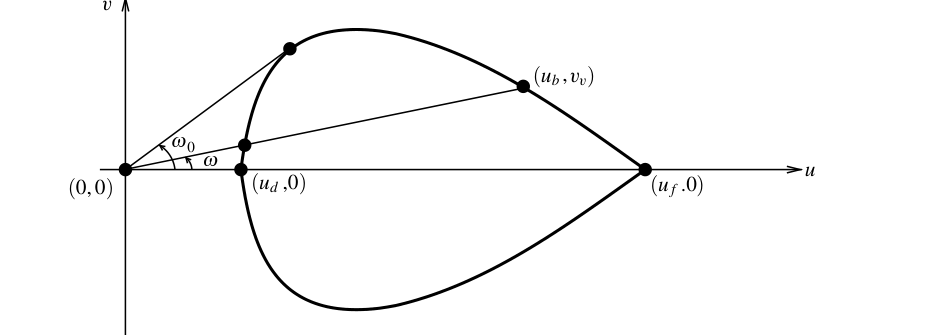
\includegraphics[width=0.8\textwidth]{ch18-fig02-01.png}
\caption{状态 $(\rho_f,u_f,0)$ 的激波极曲线：关于 $u$ 轴对称，下半支为 1-激波曲线的投影，上半支为 3-激波曲线的投影。}
\label{figure:ch18-激波极曲线}
\end{figure}

方程\eqref{align:ch18-1829}、\eqref{align:ch18-18210}定义了状态 $(\rho_f,u_f,0)$ 的所谓激波极曲线，如图\cref{figure:ch18-激波极曲线}所示。注意该激波极曲线关于 $u$ 轴对称：其下半支是 1-激波曲线在 $u$-$v$ 平面上的投影，上半支是 3-激波曲线的投影。气流方向穿过激波时偏转的角度 $\omega=\arctan(v/u)$ 可直接从激波极曲线上读出。除 $(\rho_f,u_f,0)$ 外，1- 与 3-激波曲线还在状态 $(\rho_d,u_d,0)$ 处相遇并终止，该状态由条件 $c_0=u_f$、$\rho_du_d=\rho_fu_f$ 确定。在该点 $s=\infty$，故气流在撞击激波前后均沿 $x$ 轴方向，即与激波垂直。

激波速率的平方由\eqref{align:ch18-1829}、\eqref{align:ch18-18210}确定，为
\begin{align}
u_b^2+v_b^2=u_f^2-\frac{\rho_b^2-\rho_f^2}{\rho_b^2}c_0^2,
\label{align:ch18-18211}
\end{align}
它是 $\rho_b$ 的递减函数。我们已经知道 $(\rho_f,u_f,0)$ 超声速，且容易看出 $(\rho_d,u_d,0)$ 亚声速。又 $c^2=p'(\rho_b)$ 是 $\rho_b$ 的递增函数。于是存在 $\rho_0\in(\rho_f,\rho_d)$，具有如下性质：当前面状态为 $(\rho_f,u_f,0)$ 的任一 1- 或 3-激波，其后状态 $(\rho_b,u_b,v_b)$ 在 $\rho_b\in(\rho_0,\rho_d]$ 时为亚声速，在 $\rho_b=\rho_0$ 时为声速，在 $\rho_b\in(\rho_f,\rho_0)$ 时为超声速。

接下来在定常无旋等熵气流的框架下讨论同一问题，
\begin{align}
\partial_xv-\partial_yu=0,\qquad u=\partial_x\phi,\quad v=\partial_y\phi,
\label{align:ch18-18212}
\end{align}
其中 $\phi$ 为速度势。此时，如\cref{section:ch03-例子}所说明，通行做法是保留质量平衡方程\eqref{align:ch18-1821}$_1$，即
\begin{align}
\partial_x(\rho u)+\partial_y(\rho v)=0,
\label{align:ch18-18213}
\end{align}
但弃去动量平衡方程\eqref{align:ch18-1821}$_2$ 与\eqref{align:ch18-1821}$_3$，代之以 Bernoulli 定律（见\eqref{align:ch03-Bernoulli}）：
\begin{align}
\frac12 q^2+h(\rho)=\text{常数},\qquad q^2=u^2+v^2=|\nabla\phi|^2,
\label{align:ch18-18214}
\end{align}
其中 $h=\varepsilon+p/\rho$ 为焓，其导数 $h'(\rho)=p'(\rho)/\rho$。注意当密度与速度 Lipschitz 时\eqref{align:ch18-1821}$_{2,3}$ 仍成立；即使在有激波处它们失效，$(\rho u^2+p,\rho uv)$ 与 $(\rho uv,\rho v^2+p)$ 仍构成熵--通量对，在用补偿紧致方法处理方程组时有用。这一观察还意味着：当以\eqref{align:ch18-18214}替代\eqref{align:ch18-1821}$_{2,3}$ 时，动量在激波强度的三阶精度上仍平衡；因而在弱激波流动的语境下，误差可视为可忽略。

当存在斜率 $\mathrm{d}y/\mathrm{d}x=s$ 的激波时，跳跃条件取形式
\begin{align}
[\![\phi]\!]=0,
\label{align:ch18-18215}
\end{align}
\begin{align}
s[\![\rho u]\!]=[\![\rho v]\!],
\label{align:ch18-18216}
\end{align}
\begin{align}
\left[\!\left[\frac12 q^2+h(\rho)\right]\!\right]=0.
\label{align:ch18-18217}
\end{align}
注意\eqref{align:ch18-18212}蕴涵跳跃条件
\begin{align}
s[\![v]\!]=-[\![u]\!],
\label{align:ch18-18218}
\end{align}
故速度的切向分量跨过激波连续。如\cref{section:ch03-例子}早已指出，\eqref{align:ch18-18218}意味着涡旋面与无旋流动不相容。然而我们仍可有 1- 与 3-激波，只需满足可容性条件 $[\![\rho]\!]<0$。

现在在无旋流动的设定下考察前面讨论过的构型，即可容的 1- 与 3-激波，其后状态为 $(\rho_b,u_b,v_b)$，前面状态给定为 $(\rho_f,u_f,0)$，其中 $u_f>0$。跳跃条件\eqref{align:ch18-18218}、\eqref{align:ch18-18216} 与\eqref{align:ch18-18217} 此时取形式
\begin{align}
\begin{cases}
-sv_b=u_b-u_f\\
s(\rho_fu_f-\rho_bu_b)=-\rho_bv_b\\
\frac12 u_f^2+h(\rho_f)=\frac12(u_b^2+v_b^2)+h(\rho_b).
\end{cases}
\label{align:ch18-18219}
\end{align}
同前，我们以 $\rho_b$ 参数化 1- 与 3-激波曲线的（可容分支）。令
\begin{align}
c_1^2=2[h(\rho_b)-h(\rho_f)],
\label{align:ch18-18220}
\end{align}
由\eqref{align:ch18-18219}得
\begin{align}
s=\pm c_1\left[\frac{\rho_b^2-\rho_f^2}{\rho_b^2}u_f^2-c_1^2\right]^{-\frac12},
\label{align:ch18-18221}
\end{align}
\begin{align}
u_b=u_f-\frac{\rho_b}{\rho_b+\rho_f}\frac{c_1^2}{u_f},
\label{align:ch18-18222}
\end{align}
\begin{align}
v_b^2=\left(\frac{\rho_b}{\rho_b+\rho_f}\right)^2\left[\frac{\rho_b^2-\rho_f^2}{\rho_b^2}u_f^2-c_1^2\right]\frac{c_1^2}{u_f^2}.
\label{align:ch18-18223}
\end{align}
方程\eqref{align:ch18-18222}、\eqref{align:ch18-18223} 确定了无旋流动中 $(\rho_f,u_f,0)$ 的激波极曲线。它与前面讨论的非无旋流动激波极曲线形式相似，故此处仍以\cref{figure:ch18-激波极曲线}表示。1- 与 3-激波曲线相遇并终止的状态 $(\rho_d,u_d,0)$，现由 $c_1^2=(1-\rho_f^2/\rho_d^2)u_f^2$ 与 $\rho_du_d=\rho_fu_f$ 确定。在该点 $s=\infty$，激波与气流方向垂直。代替\eqref{align:ch18-18211}，现有
\begin{align}
u_b^2+v_b^2=u_f^2-c_1^2
\label{align:ch18-18224}
\end{align}
故同样存在 $\rho_0\in(\rho_f,\rho_d)$，使 $(\rho_b,u_b,v_b)$ 在 $\rho_b\in(\rho_0,\rho_d]$ 时亚声速，在 $\rho_b=\rho_0$ 时声速，在 $\rho_b\in(\rho_f,\rho_0)$ 时超声速。

上述内容的应用将在\cref{section:ch18-超声速绕凸角}中给出。

\end{document}
